\documentclass[12pt,reqno]{amsart}

\usepackage[margin=1in]{geometry} % 1‑inch margins all around
\usepackage{setspace}             % spacing control
\doublespacing                    % turn on double‑spacing



\usepackage{amssymb,latexsym,mathrsfs,amsmath}
\usepackage{amsthm}
\usepackage{graphicx}
\usepackage{diagbox}
\usepackage{mathrsfs}
\usepackage{tikz}
\usepackage{enumitem}
\usepackage{hyperref}

\usetikzlibrary{matrix}
\usetikzlibrary{arrows}

\newtheorem{lemma}{Lemma}[section]
\newtheorem{proposition}[lemma]{Proposition}
\newtheorem{theorem}[lemma]{Theorem}
\newtheorem{corollary}[lemma]{Corollary}
\newtheorem{conjecture}[lemma]{Conjecture}

\theoremstyle{definition}
\newtheorem{remark}[lemma]{Remark}
\newtheorem{definition}[lemma]{Definition}
\newtheorem{example}[lemma]{Example}
\newtheorem{convention}[lemma]{Convention}
\newtheorem{question}[lemma]{Question}

%to make the correct symbol for Sha
%\newcommand\cyr{%
%\renewcommand\rmdefault{wncyr}%
%\renewcommand\sfdefault{wncyss}%
%\renewcommand\encodingdefault{OT2}%
%\normalfont \selectfont} \DeclareTextFontCommand{\textcyr}{\cyr}


\DeclareMathOperator{\ab}{ab}
\newcommand{\absgal}{\G_{\bbQ}}
\DeclareMathOperator{\ad}{ad}
\DeclareMathOperator{\adj}{adj}
\DeclareMathOperator{\alg}{alg}
\DeclareMathOperator{\Alt}{Alt}
\DeclareMathOperator{\Ann}{Ann}
\DeclareMathOperator{\arith}{arith}
\DeclareMathOperator{\Aut}{Aut}
\DeclareMathOperator{\Be}{B}
\DeclareMathOperator{\Bd}{Bd}
\DeclareMathOperator{\card}{card}
\DeclareMathOperator{\Char}{char}
\DeclareMathOperator{\csp}{csp}
\DeclareMathOperator{\codim}{codim}
\DeclareMathOperator{\coker}{coker}
\DeclareMathOperator{\coh}{H}
\DeclareMathOperator{\compl}{compl}
\DeclareMathOperator{\conj}{conj}
\DeclareMathOperator{\cont}{cont}
\DeclareMathOperator{\Cov}{Cov}
\DeclareMathOperator{\crys}{crys}
\DeclareMathOperator{\Crys}{Crys}
\DeclareMathOperator{\cusp}{cusp}
\DeclareMathOperator{\diag}{diag}
\DeclareMathOperator{\diam}{diam}
\DeclareMathOperator{\Dom}{Dom}
\DeclareMathOperator{\disc}{disc}
\DeclareMathOperator{\dist}{dist}
\DeclareMathOperator{\dR}{dR}
\DeclareMathOperator{\Eis}{Eis}
\DeclareMathOperator{\End}{End}
\DeclareMathOperator{\ev}{ev}
\DeclareMathOperator{\eval}{eval}
\DeclareMathOperator{\Eq}{Eq}
\DeclareMathOperator{\Ext}{Ext}
\DeclareMathOperator{\Fil}{Fil}
\DeclareMathOperator{\Fitt}{Fitt}
\DeclareMathOperator{\Frob}{Frob}
\DeclareMathOperator{\G}{G}
\DeclareMathOperator{\Gal}{Gal}
\DeclareMathOperator{\GL}{GL}
\DeclareMathOperator{\Gr}{Gr}
\DeclareMathOperator{\Graph}{Graph}
\DeclareMathOperator{\GSp}{GSp}
\DeclareMathOperator{\GUn}{GU}
\DeclareMathOperator{\Hom}{Hom}
\DeclareMathOperator{\id}{id}
\DeclareMathOperator{\Id}{Id}
\DeclareMathOperator{\Ik}{Ik}
\DeclareMathOperator{\IM}{Im}
\DeclareMathOperator{\Image}{im}
\DeclareMathOperator{\Ind}{Ind}
\DeclareMathOperator{\Inf}{inf}
\DeclareMathOperator{\Isom}{Isom}
\DeclareMathOperator{\J}{J}
\DeclareMathOperator{\Jac}{Jac}
\DeclareMathOperator{\lcm}{lcm}
\DeclareMathOperator{\length}{length}
\DeclareMathOperator*{\limit}{limit}
\DeclareMathOperator{\Log}{Log}
\DeclareMathOperator{\M}{M}
\DeclareMathOperator{\Mat}{Mat}
\DeclareMathOperator{\N}{N}
\DeclareMathOperator{\Nm}{Nm}
\DeclareMathOperator{\NIk}{N-Ik}
\DeclareMathOperator{\NSK}{N-SK}
\DeclareMathOperator{\new}{new}
\DeclareMathOperator{\obj}{obj}
\DeclareMathOperator{\old}{old}
\DeclareMathOperator{\ord}{ord}
\DeclareMathOperator{\Or}{O}
\DeclareMathOperator{\op}{op}
\DeclareMathOperator{\PGL}{PGL}
\DeclareMathOperator{\PGSp}{PGSp}
\DeclareMathOperator{\rank}{rank}
\DeclareMathOperator{\Ran}{Ran}
\DeclareMathOperator{\Rel}{Rel}
\DeclareMathOperator{\Real}{Re}
\DeclareMathOperator{\RES}{res}
\DeclareMathOperator{\Res}{Res}
%\DeclareMathOperator{\Sha}{\textcyr{Sh}}
\DeclareMathOperator{\Sel}{Sel}
\DeclareMathOperator{\semi}{ss}
\DeclareMathOperator{\sgn}{sign}
\DeclareMathOperator{\SK}{SK}
\DeclareMathOperator{\SL}{SL}
\DeclareMathOperator{\SO}{SO}
\DeclareMathOperator{\Sp}{Sp}
\DeclareMathOperator{\Span}{span}
\DeclareMathOperator{\Spec}{Spec}
\DeclareMathOperator{\spin}{spin}
\DeclareMathOperator{\st}{st}
\DeclareMathOperator{\St}{St}
\DeclareMathOperator{\SUn}{SU}
\DeclareMathOperator{\supp}{supp}
\DeclareMathOperator{\Sup}{sup}
\DeclareMathOperator{\Sym}{Sym}
\DeclareMathOperator{\Tam}{Tam}
\DeclareMathOperator{\tors}{tors}
\DeclareMathOperator{\tr}{tr}
\DeclareMathOperator{\Tr}{Tr}
\DeclareMathOperator{\un}{un}
\DeclareMathOperator{\Un}{U}
\DeclareMathOperator{\val}{val}
\DeclareMathOperator{\vol}{vol}

\DeclareMathOperator{\Sets}{S \mkern1.04mu e \mkern1.04mu t \mkern1.04mu s}
    \newcommand{\cSets}{\scalebox{1.02}{\contour{black}{$\Sets$}}}
    
\DeclareMathOperator{\Groups}{G \mkern1.04mu r \mkern1.04mu o \mkern1.04mu u \mkern1.04mu p \mkern1.04mu s}
    \newcommand{\cGroups}{\scalebox{1.02}{\contour{black}{$\Groups$}}}

\DeclareMathOperator{\TTop}{T \mkern1.04mu o \mkern1.04mu p}
    \newcommand{\cTop}{\scalebox{1.02}{\contour{black}{$\TTop$}}}

\DeclareMathOperator{\Htp}{H \mkern1.04mu t \mkern1.04mu p}
    \newcommand{\cHtp}{\scalebox{1.02}{\contour{black}{$\Htp$}}}

\DeclareMathOperator{\Mod}{M \mkern1.04mu o \mkern1.04mu d}
    \newcommand{\cMod}{\scalebox{1.02}{\contour{black}{$\Mod$}}}

\DeclareMathOperator{\Ab}{A \mkern1.04mu b}
    \newcommand{\cAb}{\scalebox{1.02}{\contour{black}{$\Ab$}}}

\DeclareMathOperator{\Rings}{R \mkern1.04mu i \mkern1.04mu n \mkern1.04mu g \mkern1.04mu s}
    \newcommand{\cRings}{\scalebox{1.02}{\contour{black}{$\Rings$}}}

\DeclareMathOperator{\ComRings}{C \mkern1.04mu o \mkern1.04mu m \mkern1.04mu R \mkern1.04mu i \mkern1.04mu n \mkern1.04mu g \mkern1.04mu s}
    \newcommand{\cComRings}{\scalebox{1.05}{\contour{black}{$\ComRings$}}}

\DeclareMathOperator{\hHom}{H \mkern1.04mu o \mkern1.04mu m}
    \newcommand{\cHom}{\scalebox{1.02}{\contour{black}{$\hHom$}}}

\renewcommand{\k}{\kappa}
\newcommand{\Ff}{F_{f}}
%\newcommand{\ts}{\,^{t}\!}


%Mathcal
\newcommand{\cA}{\mathcal{A}}
\newcommand{\cB}{\mathcal{B}}
\newcommand{\cC}{\mathcal{C}}
\newcommand{\cD}{\mathcal{D}}
\newcommand{\cE}{\mathcal{E}}
\newcommand{\cF}{\mathcal{F}}
\newcommand{\cG}{\mathcal{G}}
\newcommand{\cH}{\mathcal{H}}
\newcommand{\cI}{\mathcal{I}}
\newcommand{\cJ}{\mathcal{J}}
\newcommand{\cK}{\mathcal{K}}
\newcommand{\cL}{\mathcal{L}}
\newcommand{\cM}{\mathcal{M}}
\newcommand{\cN}{\mathcal{N}}
\newcommand{\cO}{\mathcal{O}}
\newcommand{\cP}{\mathcal{P}}
\newcommand{\cQ}{\mathcal{Q}}
\newcommand{\cR}{\mathcal{R}}
\newcommand{\cS}{\mathcal{S}}
\newcommand{\cT}{\mathcal{T}}
\newcommand{\cU}{\mathcal{U}}
\newcommand{\cV}{\mathcal{V}}
\newcommand{\cW}{\mathcal{W}}
\newcommand{\cX}{\mathcal{X}}
\newcommand{\cY}{\mathcal{Y}}
\newcommand{\cZ}{\mathcal{Z}}


%mathfrak (missing \fi)
\newcommand{\fa}{\mathfrak{a}}
\newcommand{\fA}{\mathfrak{A}}
\newcommand{\fb}{\mathfrak{b}}
\newcommand{\fB}{\mathfrak{B}}
\newcommand{\fc}{\mathfrak{c}}
\newcommand{\fC}{\mathfrak{C}}
\newcommand{\fd}{\mathfrak{d}}
\newcommand{\fD}{\mathfrak{D}}
\newcommand{\fe}{\mathfrak{e}}
\newcommand{\fE}{\mathfrak{E}}
\newcommand{\ff}{\mathfrak{f}}
\newcommand{\fF}{\mathfrak{F}}
\newcommand{\fg}{\mathfrak{g}}
\newcommand{\fG}{\mathfrak{G}}
\newcommand{\fh}{\mathfrak{h}}
\newcommand{\fH}{\mathfrak{H}}
\newcommand{\fI}{\mathfrak{I}}
\newcommand{\fj}{\mathfrak{j}}
\newcommand{\fJ}{\mathfrak{J}}
\newcommand{\fk}{\mathfrak{k}}
\newcommand{\fK}{\mathfrak{K}}
\newcommand{\fl}{\mathfrak{l}}
\newcommand{\fL}{\mathfrak{L}}
\newcommand{\fm}{\mathfrak{m}}
\newcommand{\fM}{\mathfrak{M}}
\newcommand{\fn}{\mathfrak{n}}
\newcommand{\fN}{\mathfrak{N}}
\newcommand{\fo}{\mathfrak{o}}
\newcommand{\fO}{\mathfrak{O}}
\newcommand{\fp}{\mathfrak{p}}
\newcommand{\fP}{\mathfrak{P}}
\newcommand{\fq}{\mathfrak{q}}
\newcommand{\fQ}{\mathfrak{Q}}
\newcommand{\fr}{\mathfrak{r}}
\newcommand{\fR}{\mathfrak{R}}
\newcommand{\fs}{\mathfrak{s}}
\newcommand{\fS}{\mathfrak{S}}
\newcommand{\ft}{\mathfrak{t}}
\newcommand{\fT}{\mathfrak{T}}
\newcommand{\fu}{\mathfrak{u}}
\newcommand{\fU}{\mathfrak{U}}
\newcommand{\fv}{\mathfrak{v}}
\newcommand{\fV}{\mathfrak{V}}
\newcommand{\fw}{\mathfrak{w}}
\newcommand{\fW}{\mathfrak{W}}
\newcommand{\fx}{\mathfrak{x}}
\newcommand{\fX}{\mathfrak{X}}
\newcommand{\fy}{\mathfrak{y}}
\newcommand{\fY}{\mathfrak{Y}}
\newcommand{\fz}{\mathfrak{z}}
\newcommand{\fZ}{\mathfrak{Z}}


%mathbf
\newcommand{\bfA}{\mathbf{A}}
\newcommand{\bfB}{\mathbf{B}}
\newcommand{\bfC}{\mathbf{C}}
\newcommand{\bfD}{\mathbf{D}}
\newcommand{\bfE}{\mathbf{E}}
\newcommand{\bfF}{\mathbf{F}}
\newcommand{\bfG}{\mathbf{G}}
\newcommand{\bfH}{\mathbf{H}}
\newcommand{\bfI}{\mathbf{I}}
\newcommand{\bfJ}{\mathbf{J}}
\newcommand{\bfK}{\mathbf{K}}
\newcommand{\bfL}{\mathbf{L}}
\newcommand{\bfM}{\mathbf{M}}
\newcommand{\bfN}{\mathbf{N}}
\newcommand{\bfO}{\mathbf{O}}
\newcommand{\bfP}{\mathbf{P}}
\newcommand{\bfQ}{\mathbf{Q}}
\newcommand{\bfR}{\mathbf{R}}
\newcommand{\bfS}{\mathbf{S}}
\newcommand{\bfT}{\mathbf{T}}
\newcommand{\bfU}{\mathbf{U}}
\newcommand{\bfV}{\mathbf{V}}
\newcommand{\bfW}{\mathbf{W}}
\newcommand{\bfX}{\mathbf{X}}
\newcommand{\bfY}{\mathbf{Y}}
\newcommand{\bfZ}{\mathbf{Z}}

\newcommand{\bfa}{\mathbf{a}}
\newcommand{\bfb}{\mathbf{b}}
\newcommand{\bfc}{\mathbf{c}}
\newcommand{\bfd}{\mathbf{d}}
\newcommand{\bfe}{\mathbf{e}}
\newcommand{\bff}{\mathbf{f}}
\newcommand{\bfg}{\mathbf{g}}
\newcommand{\bfh}{\mathbf{h}}
\newcommand{\bfi}{\mathbf{i}}
\newcommand{\bfj}{\mathbf{j}}
\newcommand{\bfk}{\mathbf{k}}
\newcommand{\bfl}{\mathbf{l}}
\newcommand{\bfm}{\mathbf{m}}
\newcommand{\bfn}{\mathbf{n}}
\newcommand{\bfo}{\mathbf{o}}
\newcommand{\bfp}{\mathbf{p}}
\newcommand{\bfq}{\mathbf{q}}
\newcommand{\bfr}{\mathbf{r}}
\newcommand{\bfs}{\mathbf{s}}
\newcommand{\bft}{\mathbf{t}}
\newcommand{\bfu}{\mathbf{u}}
\newcommand{\bfv}{\mathbf{v}}
\newcommand{\bfw}{\mathbf{w}}
\newcommand{\bfx}{\mathbf{x}}
\newcommand{\bfy}{\mathbf{y}}
\newcommand{\bfz}{\mathbf{z}}

%blackboard bold

\newcommand{\bbA}{\mathbb{A}}
\newcommand{\bbB}{\mathbb{B}}
\newcommand{\bbC}{\mathbb{C}}
\newcommand{\bbD}{\mathbb{D}}
\newcommand{\bbE}{\mathbb{E}}
\newcommand{\bbF}{\mathbb{F}}
\newcommand{\bbG}{\mathbb{G}}
\newcommand{\bbH}{\mathbb{H}}
\newcommand{\bbI}{\mathbb{I}}
\newcommand{\bbJ}{\mathbb{J}}
\newcommand{\bbK}{\mathbb{K}}
\newcommand{\bbL}{\mathbb{L}}
\newcommand{\bbM}{\mathbb{M}}
\newcommand{\bbN}{\mathbb{N}}
\newcommand{\bbO}{\mathbb{O}}
\newcommand{\bbP}{\mathbb{P}}
\newcommand{\bbQ}{\mathbb{Q}}
\newcommand{\bbR}{\mathbb{R}}
\newcommand{\bbS}{\mathbb{S}}
\newcommand{\bbT}{\mathbb{T}}
\newcommand{\bbU}{\mathbb{U}}
\newcommand{\bbV}{\mathbb{V}}
\newcommand{\bbW}{\mathbb{W}}
\newcommand{\bbX}{\mathbb{X}}
\newcommand{\bbY}{\mathbb{Y}}
\newcommand{\bbZ}{\mathbb{Z}}
\newcommand{\jota}{\jmath}

\newcommand{\bmat}{\left( \begin{matrix}}
\newcommand{\emat}{\end{matrix} \right)}

\newcommand{\bbmat}{\left[ \begin{matrix}}
\newcommand{\ebmat}{\end{matrix} \right]}

\newcommand{\pmat}{\left( \begin{smallmatrix}}
\newcommand{\epmat}{\end{smallmatrix} \right)}

\newcommand{\lat}{\mathscr{L}}
\newcommand{\mat}[4]{\begin{pmatrix}{#1}&{#2}\\{#3}&{#4}\end{pmatrix}}
\newcommand{\ov}[1]{\overline{#1}}
\newcommand{\res}[1]{\underset{#1}{\RES}\,}
\newcommand{\up}{\upsilon}

\newcommand{\tac}{\textasteriskcentered}

%mahesh macros
\newcommand{\tm}{\textrm}

%Comments
\newcommand{\com}[1]{\vspace{5 mm}\par \noindent
\marginpar{\textsc{Comment}} \framebox{\begin{minipage}[c]{0.95
\textwidth} \tt #1 \end{minipage}}\vspace{5 mm}\par}

\newcommand{\Bmu}{\mbox{$\raisebox{-0.59ex}
  {$l$}\hspace{-0.18em}\mu\hspace{-0.88em}\raisebox{-0.98ex}{\scalebox{2}
  {$\color{white}.$}}\hspace{-0.416em}\raisebox{+0.88ex}
  {$\color{white}.$}\hspace{0.46em}$}{}}  %need graphicx and xcolor. this produces blackboard bold mu 

\newcommand{\hooktwoheadrightarrow}{%
  \hookrightarrow\mathrel{\mspace{-15mu}}\rightarrow
}

\makeatletter
\newcommand{\xhooktwoheadrightarrow}[2][]{%
  \lhook\joinrel
  \ext@arrow 0359\rightarrowfill@ {#1}{#2}%
  \mathrel{\mspace{-15mu}}\rightarrow
}
\makeatother

\renewcommand{\geq}{\geqslant}
\renewcommand{\leq}{\leqslant}
\newcommand{\midd}{\hspace{4pt}\middle|\hspace{4pt}}
    
\newcommand{\bone}{\mathbf{1}}
\newcommand{\sign}{\mathrm{sign}}
\newcommand{\eps}{\varepsilon}
\newcommand{\textui}[1]{\uline{\textit{#1}}}

%\newcommand{\ov}{\overline}
%\newcommand{\un}{\underline}
\newcommand{\fin}{\mathrm{fin}}

\newcommand{\chnum}{\titleformat
{\chapter} % command
[display] % shape
{\centering} % format
{\Huge \color{black} \shadowbox{\thechapter}} % label
{-0.5em} % sep (space between the number and title)
{\LARGE \color{black} \underline} % before-code
}

\newcommand{\chunnum}{\titleformat
{\chapter} % command
[display] % shape
{} % format
{} % label
{0em} % sep
{ \begin{flushright} \begin{tabular}{r}  \Huge \color{black}
} % before-code
[
\end{tabular} \end{flushright} \normalsize
] % after-code
}

\newcommand{\nl}{\newline \mbox{}}

\newcommand{\h}[1]{\hspace{#1pt}}

\newcommand{\littletaller}{\mathchoice{\vphantom{\big|}}{}{}{}}
\newcommand\restr[2]{{% we make the whole thing an ordinary symbol
  \left.\kern-\nulldelimiterspace % automatically resize the bar with \right
  #1 % the function
  \littletaller % pretend it's a little taller at normal size
  \right|_{#2} % this is the delimiter
  }}

\newcommand{\mtext}[1]{\hspace{6pt}\text{#1}\hspace{6pt}}

\newcommand{\lnorm}{\left\lVert}
\newcommand{\rnorm}{\right\rVert}

\newcommand{\ds}{\displaystyle}
\newcommand{\ts}{\textstyle}


\newcommand{\sfrac}[2]{{}^{#1}\mskip -5mu/\mskip -3mu_{#2}}


\makeatletter
\newcommand*{\da@rightarrow}{\mathchar"0\hexnumber@\symAMSa 4B }
\newcommand*{\da@leftarrow}{\mathchar"0\hexnumber@\symAMSa 4C }
\newcommand*{\xdashrightarrow}[2][]{%
  \mathrel{%
    \mathpalette{\da@xarrow{#1}{#2}{}\da@rightarrow{\,}{}}{}%
  }%
}
\newcommand{\xdashleftarrow}[2][]{%
  \mathrel{%
    \mathpalette{\da@xarrow{#1}{#2}\da@leftarrow{}{}{\,}}{}%
  }%
}
\newcommand*{\da@xarrow}[7]{%
  % #1: below
  % #2: above
  % #3: arrow left
  % #4: arrow right
  % #5: space left 
  % #6: space right
  % #7: math style 
  \sbox0{$\ifx#7\scriptstyle\scriptscriptstyle\else\scriptstyle\fi#5#1#6\m@th$}%
  \sbox2{$\ifx#7\scriptstyle\scriptscriptstyle\else\scriptstyle\fi#5#2#6\m@th$}%
  \sbox4{$#7\dabar@\m@th$}%
  \dimen@=\wd0 %
  \ifdim\wd2 >\dimen@
    \dimen@=\wd2 %   
  \fi
  \count@=2 %
  \def\da@bars{\dabar@\dabar@}%
  \@whiledim\count@\wd4<\dimen@\do{%
    \advance\count@\@ne
    \expandafter\def\expandafter\da@bars\expandafter{%
      \da@bars
      \dabar@ 
    }%
  }%  
  \mathrel{#3}%
  \mathrel{%   
    \mathop{\da@bars}\limits
    \ifx\\#1\\%
    \else
      _{\copy0}%
    \fi
    \ifx\\#2\\%
    \else
      ^{\copy2}%
    \fi
  }%   
  \mathrel{#4}%
}
\makeatother

\renewcommand{\div}[2]{%
  \scalebox{0.92}{$#1$}%
  \hspace{1.2pt}%
  \scalebox{1.2}{$\mid$}%
  \hspace{0.75pt}%
  \scalebox{0.92}{$#2$}%
}



\begin{document}


\parindent1.5em
\setlength\parskip{.1em}
\thispagestyle{empty}
\title{The Effect of Weather Shocks on Housing Prices in California Counties}
\author[Gianluca Crescenzo]{Gianluca Crescenzo}
%\subjclass[2020]{primary: 57K18; secondary: 57K10}
%\keywords{Odd Khovanov homology, Steenrod square}

\begin{abstract}
    Using California county data from 2010-2019, we investigate how year-to-year weather shocks shape local housing markets. We compute temperature and precipitation $z$-scores to measure deviations from each county's 1901-2000 climate, and then merge them with Census median-price data and population controls from the California Department of Finance. We estimate two panel regressions \textemdash a baseline model and another which includes county and year fixed effects. We also run several robustness checks on the baseline specification. Across all versions, unusually warmer years lead to a small rise in median prices, while precipitation shocks show no consistent effect.
\end{abstract}

\maketitle
%%%%%%%%%%%%%%%%%%%%%%%%%%%%%%%%%%%%%%%%%%%%%%%%%%%%%%%%%%%%%%%%%%%%%%%%%%%%%
\section{Introduction}
    Weather is one of the few variables that a homeowner cannot influence, yet its year-to-year changes may still have an effect on buying and selling markets. This paper investigates whether shocks in temperature and precipitation have a significant effect on median housing prices in California. We build a balanced county-level panel from 2010-2019 containing 39 counties whose populations exceed 65000, as well as track median house prices and temperature and precipitation deviations. Each deviation is expressed as a $z$-score against the county's 1901-2000 mean. As such, each deviation is directly comparable across differing counties. Population and population densities are also included to increase the precision of our estimators.

    Our hypothesis is that weather shocks, in particular temperature, raise median house prices. Warmer conditions lengthen beach seasons, lower indoor heating costs, and increase the demand for outdoor amenities. Annual weather patterns are plausibly exogenous to local real-estate, yet two concerns still arise here. Omitted variables such as school quality could be correlated with both climate and prices, resulting in a biased coefficient. Likewise, median sales figures for large and geographically diverse counties such as Los Angeles may introduce measurement error into our models. Because of this we consider robustness checks such as dropping Los Angeles County, considering only coastline counties, and including county and year fixed effects. 

    In the baseline model a one-standard deviation change in average temperatures raises the county's median house price by 10.7\%, and a similar change in average precipitation increases median house prices by 9.1\%. Both estimates are statistically significant. Removing Los Angeles County resulted in a negligible change in estimated effects compared to our baseline results, and restricting the regression to coastline counties raised the temperature effect to 11.4\% and decreased the precipitation effect to 7.7\%. After adding county and year fixed effects, however, the temperature effect dropped to 2.3\% and became insignificant at the 5 percent level. Precipitation fell to 1.6\% but remained statistically significant. These attenuated effects suggest that long-run climate conditions \textemdash as opposed to weather shocks \textemdash have a greater effect on real-estate.

    Our findings suggest that buyers do pay attention to climate, but primarily through long-run averages rather than shocks in weather. Moreover, county medians result in large heterogeneity across neighborhoods, hiding the precise relationship between weather and housing valuations.

    The remainder of this paper proceeds as follows. Section~\ref{sec:background} describes the construction of $z$-scores, its inherent benefits, as well as the importance of random variables in our specification. Section~\ref{sec:Data} explains the sources of our data and describes the summary statistics, in particular, interesting and/or important outliers. Section~\ref{sec:emp-strat} lays out the empirical strategy by explaining each of our regression equations, the role of population controls, and how fixed effects result in temperature and precipitation deviations being unbiased. Section~\ref{sec:results} presents our baseline results, robustness checks, and also includes a discussion about the statistical significance of our estimators.
%%%%%%%%%%%%%%%%%%%%%%%%%%%%%%%%%%%%%%%%%%%%%%%%%%%%%%%%%%%%%%%%%%%%%%%%%%%%%
\section{Background}\label{sec:background}

    We can formally measure temperature and precipitation shocks by computing $z$-scores of temperature and precipitation data. Let $\text{Temp}_{ct}$ denote the average temperature of county $c$ during year $t$ and $\overline{\text{Temp}_c}$ denote the historical average temperature of county $c$. The \textit{temperature $z$-score} is given by:
        \begin{equation}\label{eq:z-score}
        \begin{split}
            z\text{Temp}_{ct} = \frac{\text{Temp}_{ct} - \overline{\text{Temp}_c}}{\sigma_{\text{Temp},c}},
        \end{split}
        \end{equation} 
    where $\sigma_{\text{Temp},c}$ are the county-specific temperature standard deviations. The precipitation $z$-scores are defined similarly. Conceptually, Equation~\ref{eq:z-score} measures how many standard deviations a county's average temperature (or precipitation) differs from its long-run mean. For example, if $z\text{Temp}_{ct} = 0$, the average temperature in county $c$ during year $t$ does not deviate from the long-run historical average. Likewise, if $z\text{Precip}_{ct} = -1$, the average precipitation was one standard deviation lower than the historical average; an unusually drier year.

    There are many advantages to using $z$-scores over raw temperature and precipitation values. Converting to $z$-scores expresses each year's weather in units of that county's historical volatility, so a value of $z\text{Temp}_{ct}=1$ is equally unusual regardless of the county. Moreover, the estimated coefficient on a $z$-score directly shows the effect of a one-standard-deviation change, making the coefficients easily interpretable and dimensionless.

    Because these weather shocks are essentially random from the perspective of buyers and sellers, they provide us a source of exogenous variation, as year-to-year swings in temperature and precipitation cannot be influenced by local housing markets. This makes $z\text{Temp}_{ct}$ and $z\text{Precip}_{ct}$ valuable regressors; any estimated effect is less likely to be confounded by other economic variables. In practice, a hot, dry year could raise cooling costs, affect construction schedules, or change the desirability of outdoor amenities. Likewise, volatility in weather patterns can be closely linked with violent crime, another factor which affects housing prices. Based on these examples, we cannot pinpoint the exact channel through which weather shocks influence housing prices.
%%%%%%%%%%%%%%%%%%%%%%%%%%%%%%%%%%%%%%%%%%%%%%%%%%%%%%%%%%%%%%%%%%%%%%%%%%%%%
\section{Data}\label{sec:Data}

    This paper uses panel data on California counties from 2010 to 2019. The main independent variables are temperature and precipitation $z$-scores computed using Equation~\ref{eq:z-score}. Average temperatures ( $^{\circ}F$) and precipitation (inches) were obtained from the National Centers for Environmental Information, which also provided the 1901-2000 long-run means. The data was available for all 58 counties in California.

    The dependent variable is county median house price. The data was provided by the United States Census Bureau, but only for counties with populations greater than or equal to 65000, leaving 39 counties. County-year population levels and land areas (used to compute density) come from the California Department of Finance and \url{https://onlinecalifornia.us/countyarea.shtml}. Population and population density are included because they correlate with housing demand yet are unlikely to respond to short-term weather shocks. Omitting them would bias the estimated weather effects.

    \begin{table*}[htbp]\centering\label{table:summ-stats}
\def\sym#1{\ifmmode^{#1}\else\(^{#1}\)\fi}
\caption{Summary Statistics}
\begin{tabular}{l*{1}{cccc}}
\hline\hline
            &        Mean&          Standard Deviation&         Minimum&         Maximum\\
\hline
Year        &      2014.5&    2.875971&        2010&        2019\\
Temperature        &    60.44974&    4.511999&        50.7&        76.5\\
Historical Average Temperature   &     58.3359&      4.1331&        51.7&        72.2\\
Precipitation     &    24.43574&    17.71261&        2.06&       82.59\\
Historical Average Precipitation &    24.90051&    14.14373&        3.38&       63.39\\
County Population  &    975545.3&     1674471&       72348&    1.01e+07\\
Median House Price&    415952.6&    229061.1&      130800&     1233600\\
County Square Miles       &    2721.245&     3391.93&       46.69&     20052.5\\
Standard Deviation of Temperature     &    1.335813&    .0912748&    1.186779&    1.521001\\
Temperature $z$-score    &    1.581177&    .9970067&   -.7024201&    3.511163\\
Standard Deviation of Precipitation  &    9.357683&    4.940643&    1.295387&    19.86239\\
Precipitation $z$-score  &   -.0875689&    .9638408&   -2.207122&    2.308191\\
County Population Density&    1025.875&    2915.774&    24.72207&    18880.89\\
Log of Median House Price&    12.80108&    .5207476&    11.78142&    14.02545\\
\hline
\(N\)       &         390&            &            &            \\
\hline\hline
\end{tabular}
\end{table*}


    Within the sample, San Bernardino County is the largest by land area (approximately 20053 square miles), whereas San Francisco County is the smallest (approximately 47 square miles) and most densely populated, at roughly 189000 residents per square mile. Mendocino County has the lowest density, with about 87000 residents overall and 22 residents per square mile.

    The largest temperature $z$-score was measured from Santa Barbara County during 2014. In fact, when sorting the 390 samples by temperature deviations, the top fourteen $z$-scores were \textit{all} measured during 2014. The largest precipitation $z$-score was measured from Imperial County during 2010. The lowest precipitation $z$-score was measured from San Mateo County during 2013.

    \begin{table*}
        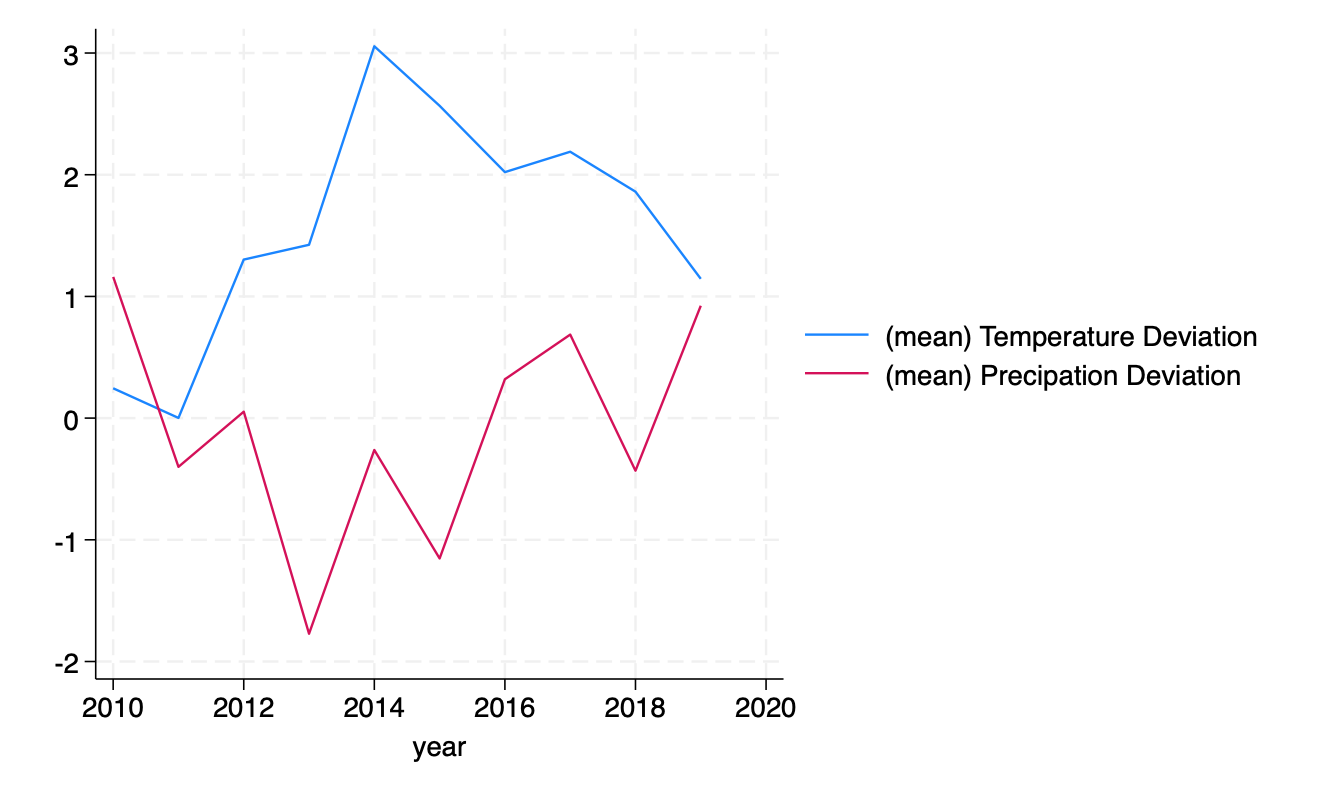
\includegraphics[scale=0.6]{avg_precip_temp_dev_year.png}
    \end{table*}

    County level data, especially in California, will inevitably hide price differences across neighborhoods in large counties. Los Angeles County, for example, spans Long Beach, Downtown L.A., Santa Clarita, and Lancaster \textemdash all of which have drastically different housing markets. Combining these into a single county-wide median will likely introduce measurement error. A better approach for future work would be to consider ZIP-code level data on median housing prices and weather patterns. Moreover, similar measurement error may be attributed to the land-area data found from the website mentioned above. Although it could be considered negligible, without knowing the accuracy or credibility of the website one can assume that any small errors will be absorbed into the error term. 

%%%%%%%%%%%%%%%%%%%%%%%%%%%%%%%%%%%%%%%%%%%%%%%%%%%%%%%%%%%%%%%%%%%%%%%%%%%%%
\section{Empirical Strategy}\label{sec:emp-strat}

    We estimate two specifications. Let $\text{Housing}_{ct}$ denote the median housing price in county $c$ during year $t$, $\text{Population}_{ct}$ the population of county $c$ during year $t$, and $\text{PopDensity}_{ct}$ the population density of county $c$ during year $t$. $z\text{Temp}_{ct}$ and $z\text{Precip}_{ct}$ are defined as per Equation~\ref{eq:z-score}. Our baseline model is:
        \begin{equation}\label{eq:reg1}
        \begin{split}
            \text{Housing}_{ct} = \beta_0 + \beta_1 z\text{Temp}_{ct} + \beta_2 z\text{Precip}_{ct} + \beta_3 \text{Population}_{ct} + \beta_4 \text{PopDensity}_{ct} + \epsilon_{ct}.
        \end{split}
        \end{equation}

    As mentioned in Section~\ref{sec:Data}, population and population density are included to increase the precision of $\beta_1$ and $\beta_2$ and help control for omitted variable bias. Table 2 shows that $\Cov(\text{Population}_{ct},z\text{Temp}_{ct})$ is non-zero with some statistical significance, so excluding population would bias the temperature coefficient.

    \begin{table}[htbp]\centering\label{table:correlation-matrix}
\def\sym#1{\ifmmode^{#1}\else\(^{#1}\)\fi}
\caption{Correlation Matrix}
\begin{tabular}{l*{4}{c}}
\hline\hline
          & Temperature        &Precipitation        &County       &County       \\
          & $z$-score        &$z$-score         &Population         &Population Density         \\
\hline
Temperature $z$-score  &        1         &                  &                  &                  \\
Precipitation $z$-score &   -0.292\sym{***}&        1         &                  &                  \\
County Population&    0.115\sym{*}  &  -0.0707         &        1         &                  \\
County Population Density&   0.0222         &  0.00637         &    0.163\sym{**} &        1         \\
\hline\hline
\multicolumn{5}{l}{\footnotesize \sym{*} \(p<0.05\), \sym{**} \(p<0.01\), \sym{***} \(p<0.001\)}\\
\end{tabular}
\end{table}



    Quality of education is a leading omitted variable: good schools raise prices, and hotter climates are often negatively correlated with education quality. If $\text{EducationQuality}_{ct}$ is omitted from Equation~\ref{eq:reg1}, and since $\Cov(\text{EducationQuality}_{ct}, \text{Housing}_{ct}) $ and \newline $\Cov(\text{EducationQuality}_{ct}, z\text{Temp}_{ct})$ are both non-zero, omitted variable bias will occur. Section~\ref{sec:results} discusses the sign and magnitude of this bias.

    Our preferred model adds county ($\alpha_c$) and year ($\delta_t$) fixed effects:
        \begin{equation}\label{eq:reg3}
        \begin{split}
            \text{Housing}_{ct} = \beta_0 + \beta_1z\text{Temp}_{ct} + \beta_2 z\text{Precip}_{ct} + \alpha_c + \delta_t + \epsilon_{ct}.
        \end{split}
        \end{equation}
    Claim: $\beta_1$ and $\beta_2$ are \textit{unbiased} estimators. Suppose $X_{ct}$ is an omitted variable from Equation~\ref{eq:reg3}. It must be the case that it is neither a time nor county fixed effect; i.e., it is something that changes within a county over time, as well as differs across counties in a given year. It cannot be $z\text{Temp}_{ct}$ or $z\text{Precip}_{ct}$ as they are both included in the regression, and similarly it must be true that $\Cov(\text{Housing}_{ct},X_{ct}) \neq 0$, $\Cov(X_{ct},z\text{Temp}_{ct}) \neq 0$, and $\Cov(X_{ct},z\text{Precip}_{ct}) \neq 0$. But how can any covariate that changes within a county over time effect weather deviations? How can any covariate which differs across counties in a given year have an effect on weather deviations? It must be the case that $\Cov(X_{ct},z\text{Temp}_{ct}) = \Cov(X_{ct},z\text{Precip}_{ct}) = 0$, giving that $X_{ct}$ is not an omitted variable. 

    Note that including county year fixed effects is expected to raise the specifications $R^2$. The inclusion of fixed effects alone will capture much of the cross-sectional and time-series variation in housing prices, so the overall $R^2$ is expected to be high.
%%%%%%%%%%%%%%%%%%%%%%%%%%%%%%%%%%%%%%%%%%%%%%%%%%%%%%%%%%%%%%%%%%%%%%%%%%%%%
\section{Results}\label{sec:results}

    

    Our null-hypothesis for each of our regression equations is that temperature and precipitation do not affect median housing prices, which we denote as:
        \begin{equation*}
        \begin{split}
            H_0: \beta_1,\beta_2 = 0.
        \end{split}
        \end{equation*}
    A failure to reject this hypothesis would indicate that temperature and precipitation deviations do not have any effect on our outcome variable. Rejecting the null-hypothesis in favour of our alternate hypothesis:
        \begin{equation*}
        \begin{split}
            H_a:\beta_1,\beta_2 \neq 0,
        \end{split}
        \end{equation*}
    indicates that there is a relationship between weather deviations and median housing prices. 

    {
\begin{table}[htbp]\centering\label{table:main_panel_results}
\def\sym#1{\ifmmode^{#1}\else\(^{#1}\)\fi}
\caption{Baseline Panel Results}
\begin{tabular}{l*{3}{c}}
    \hline\hline
 \scalebox{0.9}{Dependent variable is the}                   \\
\scalebox{0.9}{log of median house prices}                    &\multicolumn{1}{c}{(1)}\\
                    \hline
Temperature $z$-score           &       0.107\sym{***}\\
                                &     (0.024)         \\
Precipitation $z$-score         &       0.091\sym{***}\\
                                &     (0.025)         \\
County Population               &       0.000\sym{***}\\
                                &     (0.000)         \\
County Population Density       &       0.000\sym{***}\\
                                &     (0.000)         \\

Constant                        &      12.530\sym{***}\\
                                &     (0.042)         \\
                    \hline
Observations                    &         390         \\
$R^2$                           &       0.237         \\
\hline\hline
{\footnotesize \sym{*} \(p<0.05\), \sym{**} \(p<0.01\), \sym{***} \(p<0.001\)}\\
\end{tabular}
\end{table}
}


    In our baseline model, a one-standard-deviation increase in average temperatures raises median house prices by 10.7\%, while a similar change in precipitation raises them by 9.1\%. Both coefficients are statistically significant at the $p < 0.001$ level, and as such we can reject the null-hypothesis that temperature and precipitation deviations do not have an effect on median housing prices. At California's 2019 county median of roughly \$500000, an 11\% increase adds \$55000, a substantial increase. Although significant at $p<0.001$, county population and population density have little to no effect. Excluding them yields $\widehat{\beta_1}=0.11894$ and $\widehat{\beta_2}=0.09053$, showing that bias from these controls is negligible.

    {
\begin{table}[htbp]\centering\label{table:main_panel_results}
\def\sym#1{\ifmmode^{#1}\else\(^{#1}\)\fi}
\caption{Robust Results}
\begin{tabular}{l*{3}{c}}
    \hline\hline
 \scalebox{0.9}{Dependent variable is the}                   &\multicolumn{1}{c}{(1) Coastline }&\multicolumn{1}{c}{(2) Exclude}&\multicolumn{1}{c}{(3) County \& Year}\\
\scalebox{0.9}{log of median house prices}                    &\multicolumn{1}{c}{Counties}&\multicolumn{1}{c}{Los Angeles}&\multicolumn{1}{c}{Fixed Effects}\\
                    \hline
Temperature $z$-score           &       0.114\sym{***}&       0.101\sym{***}&       0.023         \\
                                &     (0.024)         &     (0.024)         &     (0.014)         \\
Precipitation $z$-score         &       0.077\sym{***}&       0.090\sym{***}&       0.016\sym{**} \\
                                &     (0.025)         &     (0.026)         &     (0.007)         \\
County Population               &       0.000\sym{***}&       0.000\sym{***}&        \\
                                &     (0.000)         &     (0.000)         &              \\
County Population Density       &       0.000\sym{***}&       0.000\sym{***}&         \\
                                &     (0.000)         &     (0.000)         &              \\
Year=2010                       &                     &                     &       0.000         \\
                                &                     &                     &         (.)         \\
Year=2011                       &                     &                     &      -0.045\sym{**} \\
                                &                     &                     &     (0.017)         \\
Year=2012                       &                     &                     &      -0.109\sym{***}\\
                                &                     &                     &     (0.016)         \\
Year=2013                       &                     &                     &      -0.022         \\
                                &                     &                     &     (0.018)         \\
Year=2014                       &                     &                     &       0.010         \\
                                &                     &                     &     (0.034)         \\
Year=2015                       &                     &                     &       0.123\sym{***}\\
                                &                     &                     &     (0.029)         \\
Year=2016                       &                     &                     &       0.176\sym{***}\\
                                &                     &                     &     (0.030)         \\
Year=2017                       &                     &                     &       0.240\sym{***}\\
                                &                     &                     &     (0.031)         \\
Year=2018                       &                     &                     &       0.326\sym{***}\\
                                &                     &                     &     (0.030)         \\
Year=2019                       &                     &                     &       0.366\sym{***}\\
                                &                     &                     &     (0.026)         \\
Constant                        &      12.946\sym{***}&      12.498\sym{***}&      12.113\sym{***}\\
                                &     (0.049)         &     (0.044)         &     (0.225)         \\
                    \hline
Observations                    &         190         &         380         &         390         \\
$R^2$                           &       0.274         &       0.243         &       0.990         \\
\hline\hline
{\footnotesize \sym{*} \(p<0.05\), \sym{**} \(p<0.01\), \sym{***} \(p<0.001\)}\\
\end{tabular}
\end{table}
}


    For robustness we consider two separate panel regressions, one which drops Los Angeles County and one which restricts the sample to coastline counties. For coastline counties, a $+1$ temperature $z$-score raises prices by 11.4\% (0.7 percentage points higher than the baseline). A unit increase in precipitation $z$-scores leads to a 7.7\% rise (1.3 percentage points lower than the baseline). Excluding Los Angeles County gives negligible changes, indicating that our results are not driven by an outlier county. All specifications still produced statistically significant estimates at $p < 0.001$; we therefore continue to reject the null hypothesis that weather deviations have no effect on housing prices.

    As mentioned in Section~\ref{sec:emp-strat}, including county and year fixed effects makes $\beta_1$ and $\beta_2$ \textit{unbiased}. Any county-level covariate that is time-invariant \textemdash for example, distance to the coast \textemdash gets absorbed, meaning that our estimators for Equation~\ref{eq:reg1} are over-biased. The same is true for any covariate which gets picked up by year fixed effects. Our $\widehat{\beta_1}$ and $\widehat{\beta_2}$ estimators for Equation~\ref{eq:reg3} can be considered negligible \textemdash a one standard deviation change in average temperatures leads to a 2.3\% increase in median housing prices, whilst a one standard deviation change in average precipitation leads to a 1.6\% increase in median housing prices. We are unable to reject the null hypothesis for $\widehat{\beta_1}$ at the $p<0.05$ level, while we can reject the null hypothesis for $\widehat{\beta_2}$ at the $p<0.01$ level. Every year, excluding 2013 and 2014, was statistically significant at the $p<0.001$ level. This is quite surprising, as we mentioned in Section~\ref{sec:Data} that 2014 was an unusually warmer and dryer year compared to its long-run historical average.

    There are many reasons why statistical significance disappears once fixed effects are added. County fixed effects remove every time-invariant county trait, so $\widehat{\beta_1}$ now relies only on within-county year-to-year variation, which is much smaller. Moreover, our $z$-scores are defined against the 1901-2000 mean, but the sample covers only 2010-2019, leaving limited variation after fixed effects. Ultimately, the inclusion of fixed effects was able to remove bias from omitted variables at the cost of statistical significance. With less variation in our regression equation, the estimated effect of $\widehat{\beta_1}$ is both smaller and \textemdash despite the standard error falling from 0.024 to 0.014 \textemdash no longer large enough relative to its standard error to reject at the $p < 0.05$ level.
%%%%%%%%%%%%%%%%%%%%%%%%%%%%%%%%%%%%%%%%%%%%%%%%%%%%%%%%%%%%%%%%%%%%%%%%%%%%%
\section{Conclusion}

    Our analysis in this paper shows that weather deviations have an effect on California's housing market, but only modestly and not always robustly. In the baseline specification, a one-standard-deviation increase in average temperatures raised county's median house prices by roughly 11\%, while the effect of precipitation is similar in magnitude but less stable. These results pass several robustness checks \textemdash including dropping Los Angeles County, and focusing only on coastline counties. However, our results shrink drastically once county and year fixed effects are included, where county temperature deviations raise prices by only 2-3\% and lose statistical significance. Taken together, the evidence suggests that long-run county climate differences, rather than short-term weather shocks, have a greater effect on median housing prices. Because county-level median prices potentially lead to measurement error, future work could clarify this by using ZIP code level data to better understand the climate component of median housing prices.
%%%%%%%%%%%%%%%%%%%%%%%%%%%%%%%%%%%%%%%%%%%%%%%%%%%%%%%%%%%%%%%%%%%%%%%%%%%%%
\bibliography{KnotHomology}
\bibliographystyle{amsalpha}

\end{document}